
%
%  $Description: Project Final Report for CSE 825$
%
%  $Authors: Vince Fasburg, Bonnie Reiff, Josh Thomas $
%  $Date: 2015/04/13 $
%  $Revision: 1.1 $
%

%\documentclass{ieee}
\documentclass[pagenumbers]{ieee}

%------------------------------------------------------------------------- 
%
% to produce page numbers, bottom centered, in the output. Default is 
% no page numbers for camera-ready copy.
%
%------------------------------------------------------------------------- 

\usepackage{times}
\usepackage{graphicx}

\begin{document}

\title{CSE 825: Project Final Report \\
USB Keyboard and Mouse Spoofing\\
}

\author{Vince Fasburg, Bonnie Reiff, and Josh Thomas\\
Dept of Computer Science and Engineering, Michigan State University\\
East Lansing, MI, USA\\
\{Vincent.Fasburg, Bonnie.Reiff, Josh.Thomas\}@ge.com\\
}

\maketitle
\thispagestyle{empty}

%------------------------------------------------------------------------- 
\section{Overview}

Universal Serial Bus (USB) technology has become ubiquitous within our society since the turn of the twenty-first century. This type of the connection has become the standard for computer peripherals such as keyboards, mouses, printers, and external disk drives. USB has also become a common method of connecting devices such as smart phones and digital cameras to computers for power supply and media transfer. It is important for this project to note that all hardware attached to the computer via USB (and other protocols as well) requires an individual device driver in order to enable communication with the computer. Device drivers provide a software interface between the computer and the hardware, allowing the computer to access functions without knowing the exact details of the hardware. Typically, installation of a new device driver is the only obvious notification from a computer desktop that a USB device has been plugged into the computer \textemdash{} the operating system will not ask the user if he or she wishes to allow the device.

This project will focus on the emulation of Human Interface Devices (HIDs), specifically a keyboard and a mouse, through the use of a programmable microcontroller (the Teensy). More will be explained about how this emulation is possible in the ``Approach" section of this report. The future findings of this project can be extended to other USB-connected devices as well, as demonstrated by Karsten Nohl and Jakob Lell at the Black Hat USA Conference in 2014 when they reprogrammed a USB flash memory device to emulate HIDs \cite{nohl}. Through use of keyboard commands and shell scripting, as well as mouse automation to interact with GUI elements, the microcontroller can essentially perform any task available for the current privilege level of the system within seconds, unbeknownst to to user. In order to launch these attacks, the malicious hacker need only plug in the USB device for a short amount of time. For example, this can be done if a user leaves a computer unlocked. Alternatively, the malicious hacker may get the user to plug the device in themselves, as users tend to have a trust that USB devices will not run any programs on their computers without their consent.

%This class of attacks is potentially very dangerous because once the program has the ability to the use the keyboard and mouse, a Linux terminal can be opened to do almost anything to the system, for example, ``rm -rf *'' which would recursively wipes all of the files from the current directory on the drive. The program could easily run without the user being aware since a terminal window could be opened up and immediately minimized while the program is still running. After only a few seconds, the program could be finished running and have the terminal window closed all before the user realizes anything is wrong.

With this background in mind, the proposed project has the goal of answering three questions through both research and implementation:

\begin{enumerate}
\item \textit{What is the extent of attacks the can be performed using USB-HID emulation?}

Initial research for this project has shown attacks on Windows and Apple PC operating systems that include actions such as setting up a reverse shell and changing the Domain Name System (DNS) server (see the ``Previous Work" section for full explanations and citations). The proposed project will explore how these attacks, as well as many others, can be implemented for a  Linux operating system using a programmable USB microcontroller. This suite of attacks will be also be used during the second portion of the project, in which defenses against these attacks will be explored.

\item \textit{What are the existing defenses against HID emulation attacks?}

This question is essentially answered in this project proposal in the ``Previous Work" section, but is included in the Problem Definition because it will be important to final report for the project. The goal of the project is for the team to design defenses against USB-HID emulation attacks, and thus it is important to know this information  in order to compare the approaches that have been taken on features such as feasibility, strength, etc.

\item \textit{Can drivers be designed for USB mouses and keyboards to defend against HID emulation attacks?}

This final question is the most essential and significant to the project as it will require designing and implementing a new concept for USB-HID devices, as well imagining the ways in which the newly implemented defenses can be weakened. The overall goal is to implement drivers for USB mouses and keyboards that have the ability to distinguish between emulated (malicious) devices and human-controlled devices. As will be explained in the following sections, the team has some initial ideas on how this can be done, but there are weaknesses to those ideas that will need to be overcome.

\end{enumerate}

%------------------------------------------------------------------------- 

\section{Previous Work}

The Teensy microcontroller has been used for many purposes, including mounting several different HID based attacks on various systems that accept input from USB human interface devices. An excellent resource that demonstrates the need for HID authentication is the website of Samy Kamkar \cite{samy}, in which the author shows an attack he calls ``USBDriveby''. The USBDriveby attack uses a Teensy microcontroller, emulating a keyboard and a mouse simultaneously,  to create a permanent connection to a remote server that is controlled by the attacker.  This connection will be re-established regularly so that the attacker can issue commands to the machine at any point in the future, including after the microcontroller has been disconnected from the victim's machine.

This example of an emulated HID-based attack serves to show the severity with which a system can be compromised when a malicious USB device is connected for even a short period of time, and without requiring an administrator password. Although the USBDriveby attack was created for the Apple OSX operating system, similar attacks may be possible on any other system that accepts USB input devices. The list of potential attacks is very large, including attacks with various effects to the victim, and ranging from very simple to very complex in implementation.

Although some attempts have been made to develop a mechanism for the authentication of USB devices, much less attention has been paid to the authentication of USB human interface devices. In a paper \cite{wang} proposing an extension to a USB driver to authenticate USB connections, the proposed 2-way authentication mechanism specifically excludes ``non-programmable devices'' such as a USB keyboard. This seems sensible, but leaves a system vulnerable to programmed attacks hiding inside a ``non-programmable device''.

Among the literature dealing with USB device security, some papers such as ``Plug \& Prey: Malicious USB Devices'' \cite{crenshaw} come closer to a solution regarding malicious HIDs. The paper describes how, on Windows, you can use registry changes to prevent USB devices from being installed. However, this would prevent legitimate HIDs from being installed also, unless a whitelist of vendor IDs and product IDs is used to allow certain devices. However, these properties can be spoofed, so the Teensy device may appear to be a whitelisted device.

The final suggestion in this paper is to apply settings to allow administrators to override the policy preventing the installation of a HID. This technique would run into problems if the device in question were the first HID to be connected to the machine, as the user would have no way to allow the installation. Furthermore, it requires administrative privileges to plug in a keyboard or mouse. The mechanism to disable installing USB devices is very different for Linux system, but the results and limitations are roughly the same.

A novel approach to USB authentication specifically for HIDs was proposed by Barbhuiya et al. \cite{barbhuiya}, which relies on either continuous or periodic authentication based on keystroke dynamics, including metrics such as the speed of typing, and the relative times of presses and releases of the keys. This method uses a stored profile of typing behaviors from the authentic user to determine whether the keystroke dynamics exhibited by the inputs are a match to the known patterns. If the keystroke dynamics are determined not to match the stored profile, the input will not be processed.

The keyboard dynamics approach to preventing emulated HID attacks would likely succeed most of the time. However, there are some significant drawbacks in this type of technique from a usability standpoint, stemming from both false positive and false negative authentication. Consider that an attack from a malicious device may be extremely short, and thus more likely to be unintentionally allowed through the authentication (consider the command ``rm -rf *''). If the malicious device were programmed to enter input in a human seeming way (perhaps emulating keyboard dynamics of an average human), there is a significant chance that small amounts of inputs would be accepted \cite{shahzad}. Furthermore, a user using a computer equipped with keystroke dynamics based authentication may reject input from a legitimate user if keystroke patterns change do to any variation in the environment or the user. Lastly, the principles of keyboard dynamics cannot easily be generalized to include authentication for a mouse as well as a keyboard.

Finally, at the 2014 Las Vegas Black Hat Security Conference, Karsten Nohl and Jakob Lell presented several USB based attacks that they collectively referred to as BadUSB \cite{nohl}. Among the attacks described is the malicious emulation of a HID. This section of the presentation describes how an emulated keyboard could be used to steal the administrative password on a Linux system, then allowing the device to perform other actions using the sudo command. The only defenses proposed in this presentation that would be suitable against an emulated keyboard or mouse were to block USB devices entirely, or by using a blacklist or whitelist of device types. As stated previously, such defenses can easily be overcome by spoofing a legitimate device ID.

%------------------------------------------------------------------------- 

\section{Approach}

This project includes two main parts which include first exploiting a few weaknesses in a computer system by creating a suite of attacks, then offering a solution to those weaknesses by developing a method to prevent future attacks. This section will describe the approach for each part of the project.

For the first part of the project, the team programed a Teensy microcontroller, shown in Figure~\ref{fig:Teensy}, to run a suite of attacks on a Linux operating system. The main idea was to emulate a USB keyboard and mouse with the Teensy so that the computer's Linux operating system would recognize the Teensy as a ``safe" device. This is easily achievable after installing the Arduino and Teensyduino software on the computer being used to program the Teensy using the development environment option to use a board that emulates a USB keyboard and mouse. Once the operating system believes that the Teensy is a safe device, the program can send keyboard or mouse commands to the operating system. The operating system should not notice anything different about these commands as compared to the commands coming from an actual keyboard or mouse. A broad range of attacks were created, including some which would require administrative privileges as described in further detail in Section~\ref{section:teensy}.

\begin{figure}[H]
   \center{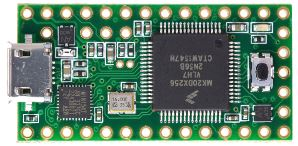
\includegraphics[width=1\linewidth]{Pictures/Teensy}}
   \caption{Teensy Microcontroller}
   \label{fig:Teensy}
\end{figure}

For the second part of the project, the team worked on preventing the attacks that were created in the first part by creating a modification to the Linux driver which handles USB devices such as a keyboard and mouse. The goal of this modification is to authenticate the USB device before any attached keyboard or mouse is allowed to be used normally.

In order to authenticate the USB device, a basic Turing test is used to determine if the input device is being used by a computer or a human. Essentially, a Turing test is a test of a machine's ability to exhibit human behavior indistinguishable of that of a human \cite{turing}. A common way to administer this test is through the use of a random text Captcha. 

The program installed on the Teensy would not know what the random captcha text is going to be, so a human user is required to type in the letters before the keyboard is allowed to be used. In addition, the mouse is verified by requiring the user to hover over the letters of the captcha on a virtual keyboard with the mouse. If the captcha is not entered correctly, the test fails and no other input is allowed from the device until the captcha is completed correctly.

%------------------------------------------------------------------------- 

\section{Threat Model}

%------------------------------------------------------------------------- 

\section{Technical Details}

%------------------------------------------------------------------------- 

\subsection{Teensy Attacks}
\label{section:teensy}

%------------------------------------------------------------------------- 

\subsection{Java GUI}
\label{section:gui}
In order for the user to validate the USB device, a Graphical User Interface (GUI) was created with a captcha and a method to validate both with the mouse and the keyboard. The GUI was created in Java with the basic components of the Java Swing \cite{kim} library as shown in Figure~\ref{fig:JavaGUI}.

\begin{figure}[H]
	\center{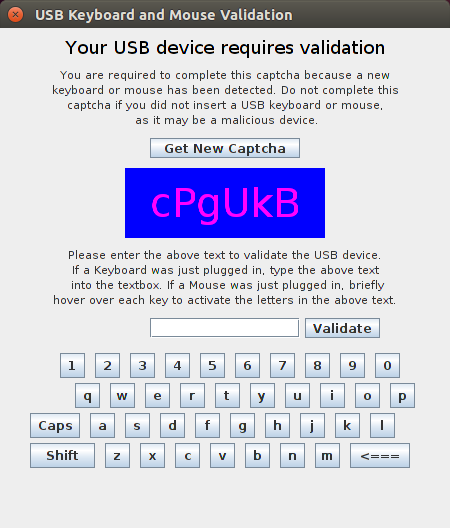
\includegraphics[width=1\linewidth]{Pictures/JavaGUI}}
	\caption{GUI to Validate USB Device}
	\label{fig:JavaGUI}
\end{figure}

The captcha was generated with a random sequence of six alphanumeric characters in both upper and lower case. The current captcha is non-web based and is generated completely with the use of a java class. The user can generate a new captcha with the ``Get New Captcha'' button in the event one of the captchas is unreadable. The background color, foreground color, and font also have the ability to be randomized with a blacklist in place to prevent certain color combinations.

The GUI has been designed to always stay on top of other windows as well as always remain in focus. This prevents a malicious program from trying to open a terminal or closing out of the GUI. In addition, each time the GUI opens, it appears in a randomized location on the screen. This location is bounded to prevent the GUI from opening up partially or fully off of the screen. This prevents an emulation program from pre-programming where the buttons on the GUI will be located then using this information to try to close it or read the captcha with some kind of computer vision. The ``x'' to close the GUI has also been disabled so the GUI can only be closed with the correct input of the captcha.

There are two methods to input the captcha text for validation. The first method would be used if a keyboard needed to be validated. The user would simply type the captcha text directly into the blank textbox and then press enter or briefly hover over the ``Validate'' button.

The second method would be used if a mouse needed to be validated. The user would use the virtual keyboard on the GUI to type the captcha into the textbox. As another security feature, clicking of the mouse has been disabled. The user would activate the keys by briefly hovering \cite{hover} over each key that is needed. When finished, the user can also briefly hover over the ``Validate'' button.

If the captcha is incorrect, an error message would appear along with a new captcha to attempt. With a correct captcha, the GUI is closed and the user gains full access of both the keyboard and mouse.

%------------------------------------------------------------------------- 

\subsection{Kernel}

The driver modification development for this paper occurred on a computer running Ubuntu 14.04 LTS with a 3.13.0-32 kernel release. The final testing of the new driver occurred within the 3.13.0-46 kernel release due to a software update. The baseline code used for the driver modification work was the latest stable kernel found on The Linux Kernel Archives website \cite{kernel}
, version 3.19.3. 

The work for the driver modification was focused entirely within the \texttt{linux-3.19/drivers/hid/usbhid} subdirectory and made use of the header files at \texttt{linux-3.19/include/linux}. The appropriate drivers for the project (usbhid, usbmouse, and usbkbd) were discovered by browsing the various subfolders of the ``drivers'' directory of the linux source code.

\subsubsection{Makefile Modification}

In order to get the driver source code in the usbhid directory to compile initially after download, several modifications had to be made. First, Makefile targets ``all'' and ``clean'' were added. The ``all'' target is set to \texttt{make -C lib/modules/\$(KVERSION)/build M=\$(PWD) modules}, where \texttt{KVERSION = \$(shell uname -r)}. Similarly, the ``clean'' target is set to \texttt{make -C /lib/modules/\$(KVERSION)/build M=\$(PWD) clean}. For any files in the directory that were still producing errors due to unrecognized information from the linux header files, the appropriate code was copied and pasted locally to eliminate compilation errors.

\subsubsection{\texttt{call\_usermodehelper} Function}

The \texttt{call\_usermodehelper} function was essential to the driver modification work. This function allows user space applications to be invoked from the kernel. The \texttt{call\_usermodehelper} function combines the functionalities of the \texttt{call\_usermodehelper\_setup} and the \texttt{call\_usermodehelper\_exec} functions, which are both part of the \texttt{usermode-helper} API. The \texttt{call\_usermodehelper\_setup} function prepares a handler for the user space call, whereas the \texttt{call\_usermodehelper\_exec} function invokes the user space call. The \texttt{call\_usermodehelper} function is defined in \texttt{linux-3.19/include/linux/kmod.h} and has four input parameters \cite{ibm}:
\begin{itemize}
\item \textit{char *path}, the path to the program to be executed
\item \textit{char **argv}, the null terminated list of program arguments, including the name of the program at zeroth index
\item \textit{char **envp}, the null terminated list containing environment information 
\item \textit{int wait}, \texttt{UMH\_WAIT\_EXEC} to wait for the user space application to be invoked before continuing, \texttt{UMH\_WAIT\_PROC} to wait for the entire process (including the application running in user space) to complete, or \texttt{UMH\_NO\_WAIT} to include no wait time
\end{itemize}

The newly implemented usage of this function in the usbhid driver is shown in Figure~\ref{fig:usermodehelper_code}.

\begin{figure}[H]
   \center{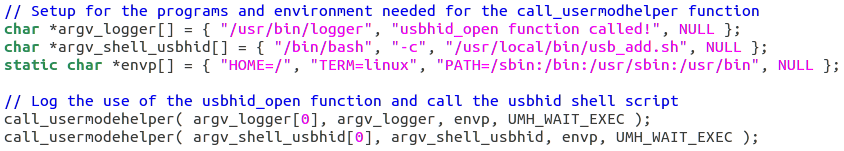
\includegraphics[width=1\linewidth]{Pictures/usermodehelper_code}}
   \caption{\texttt{call\_usermodehelper} additions to the \texttt{usbhid\_open} function}
   \label{fig:usermodehelper_code}
\end{figure}

The appropriate function to modify was then determined using the system log (found at \texttt{/var/log/syslog}). The text logged upon insertion and removal of a USB-HID device was searched within the \texttt{usbhid} directory to determine a subset of files and functions to modify. System logging calls were then added to this set of functions to choose the exact driver modification location \textemdash the \texttt{usbhid\_open} function in hid-core.c.
%TODO%%%%%%%%
TODO: discussion of system logging and calling the bash script using the function

\subsubsection{Installation of Modules}

When the kernel source files are compiled, they produce both regular C object files (.o) and loadable kernel module files (.ko). The following steps then need to be taken to install the new versions of the modules. Note that these steps were scripted as part of the project in order to allow for faster installation and test of changes:

\begin{enumerate}
\item Uninstall the old versions of the module at \texttt{/lib/modules/\$(uname -r)/kernel/ drivers/hid/usbhid} using the \texttt{sudo rmmod usbhid.ko} command
\item Copy the new module to \texttt{/lib/modules/\$(uname -r)/kernel/drivers/hid/usbhid}
\item Insert the new module using the \texttt{sudo insmod usbhid.ko} command
\end{enumerate} 

To verify the insertion or removal of a module, the \texttt{lsmod} command can be used to show the status of the modules in the Linux kernel. This program also shows the size of each module (which is helpful for distinguishing between different versions), as well as what other modules are dependent on it.

%------------------------------------------------------------------------- 

\subsection{Bash Script}

%------------------------------------------------------------------------- 

\section{Experimental Results}

After development of the modified driver was complete and installed on an Ubuntu system, the modified driver was tested against three types of devices: 

\begin{itemize}
\item \textit{USB Flash Drive.}

This test was executed to ensure that the captcha program only appears for human interface devices as opposed to for all USB devices. The computer responded as expected \textemdash a File window showing the contents of the USB flash drive was opened and the captcha program did not run.

\item \textit{USB Mouse and USB Keyboard}.

This test was executed to ensure that the captcha program runs as expected for the devices on which this research focused.

\item \textit{Teensy Programmable Microcontroller with attack loaded.}

The Teensy was loaded with each of the attacks described in Section~\ref{section:teensy} of the paper and set to emulate both a USB mouse and USB keyboard. The Teensy was subsequently plugged into a USB port and the system was observed to see what (if anything) occurred before the captcha program loaded.

\end{itemize}

%------------------------------------------------------------------------- 

\section{Usability Testing}

Usability testing is used in products that have a user-centered interaction in order to evaluate it by testing on outside users. As a part of the overall testing of the USB verification software, we had individuals who were not part of the development team use the software to see their overall impression of the design. The following summarizes  the outcomes of the study:
\begin{enumerate}
\item Users did not completely understand the idea behind hovering over the buttons to activate them. We found that some users would try to click, and then ended up hovering too long which allowed multiple letters to appear. In future versions of the Java GUI, we could reevaluate the usefulness of the hovering feature. Since the GUI does also keep its own focus and stays on top of other windows, disabling the clicking may not be required. 
\item A few individuals mentioned that the letters on the keyboard were a bit too small. If someone had bad eye sight, it would be even more difficult to see. The size of the text for the buttons should be enlarged so that it is easier to read. In addition, by enlarging the text on the keys, the keys would become larger as well. This could help users type on the keyboard more easily by making bigger targets to guide the mouse to.
\item Lastly, there were comments made on the length of the directions on the page. Most people probably do not want to take the time to read all the through them and may begin completing the captcha before having finished reading. This could lead to the captcha being completed incorrectly or using the wrong method (mouse verification vs keyboard verification). If there is some way to summarize the directions and increase the size of the font to make the user more aware of what to do, that would be very helpful.
\end{enumerate}
%------------------------------------------------------------------------- 

\section{Technical Weaknesses}
\label{section:weakness}

%------------------------------------------------------------------------- 

\section{Conclusion \& Future Work}

In this paper, we examined the following three aspects of USB-HID emulation attacks on an Ubuntu operating system:

\begin{itemize}
\item The extent of attacks the can be performed using USB-HID emulation with a programmable microcontroller
\item The existing defenses against USB-HID emulation attacks
\item New possibilities for USB-HID driver design to defend against HID emulation attacks
\end{itemize}

The resulting research produced Ubuntu attacks written for the Teensy USB-based microcontroller development system, as well as a modification to the ``usbhid'' Linux driver that has been proven to stop the Teensy-based attacks while still allowing normal use of USB input devices such as the mouse and keyboard. The driver modification in its current state runs a bash shell script to restrict keyboard and mouse functionality until a team developed captcha GUI (written in Java) is completed successfully.

As this was a proof of concept, in addition to fixing the technical weaknesses explained Section~\ref{section:weakness}, there are several improvements that can be made in future versions of the driver modification. Once such improvement would be to use a more advanced captcha. As stated in Section~\ref{section:gui}, the current captcha is a non-web based random sequence of six alphanumeric characters with randomized background color, foreground color, and font. A more advanced captcha contains characteristics such as letter distortion and strokes through the text, and makes tasks such as segmentation (the ability to spearate one letter from another) difficult, especially without understanding the context of the words \cite{captcha}.

The other two suggested improvements for future work revolve around the concept of containing all elements of the USB-HID validation to ``kernel space'', from where the shell script is initially called. Kernel space is a privileged area of virtual memory reserved for the operating system and most device drivers, whereas user space allows application software to run. Even though the shell script described in the ``Bash Script'' section of this paper is called from device driver code (kernel space), the shell script actually executes in user space, which is not preferable. In order to contain all shell script functionality within kernel space, the restriction of keyboard and mouse functions and the execution of the captcha program would both need to be converted to C code. 

Since interpreted code cannot be run in kernel space, the captcha program would need to be ported to a language other than Java or Python in order to call the program from the C code \textemdash the program would most likely still be called using the \texttt{call\_usermodehelper} function described in the ``Kernel'' section of this paper. In regards to the restriction of keyboard and mouse functions, structures exist in the code for the ``usbmouse'' and ``usbkbd'' drivers (unmodified in the scope of work for this project) that can be modified in a similar manner to how the functionality of these two devices was modified in the shell script. For the available keys on the keyboard, the ``Xmodmap'' mapping files used currently are analogous to the \texttt{usb\_kbd\_keycode} array of 256 \texttt{char} types (found in usbkbd.c), which can be changed using the \texttt{input\_report\_key} function. Similarly, the ability to use various buttons on the mouse can be restricted or unrestricted by using the \texttt{input\_report\_key} and \texttt{input\_report\_rel} functions, as seen in the \texttt{usb\_mouse\_irq} function in the usbmouse.c file.

%------------------------------------------------------------------------- 

\appendix 

%\newpage% -- remove this comment if we want the Appendix and References on a new page

\section{Appendix: Team Contributions}

The major project deliverables and testing of the end product were divided as follows among the team members:

\begin{center}
	\begin{tabular}{ | c | c | }
		\hline \textbf{Project Contribution} & \textbf{Assigned Team Member} \\ \hline
		Teensy code attacks & Vince Fasburg \\ \hline
		Captcha GUI & Josh Thomas \\ \hline
		Driver modification & Bonnie Reiff \\ \hline
		Shell script & Vince Fasburg \\ \hline
		Udev rule research & Vince Fasburg \\ \hline
		Final product testing against attacks & Bonnie Reiff \\ \hline
		Usability testing & Josh Thomas \\ \hline
	\end{tabular}
\end{center}

Each student on the team wrote about his or her own project responsibilities in the final project paper. In addition, the extra paper sections were assigned as follows:

\begin{center}
	\begin{tabular}{ | c | c | }
		\hline \textbf{Team Member} & \textbf{Extra Paper Sections} \\ \hline
		Vince Fasburg & Threat Model, Technical Weaknesses \\ \hline
		Bonnie Reiff &  Future Work \\ \hline
		Josh Thomas & Overview, Previous Work, Approach  \\ \hline
	\end{tabular}
\end{center}

 All team members were responsible for final read through and editing of the final paper.

%------------------------------------------------------------------------- 

\bibliographystyle{ieee}
\bibliography{bibfile}

\end{document}

